\documentclass[]{article}
\usepackage{lmodern}
\usepackage{amssymb,amsmath}
\usepackage{ifxetex,ifluatex}
\usepackage{fixltx2e} % provides \textsubscript
\ifnum 0\ifxetex 1\fi\ifluatex 1\fi=0 % if pdftex
  \usepackage[T1]{fontenc}
  \usepackage[utf8]{inputenc}
\else % if luatex or xelatex
  \ifxetex
    \usepackage{mathspec}
    \usepackage{xltxtra,xunicode}
  \else
    \usepackage{fontspec}
  \fi
  \defaultfontfeatures{Mapping=tex-text,Scale=MatchLowercase}
  \newcommand{\euro}{€}
\fi
% use upquote if available, for straight quotes in verbatim environments
\IfFileExists{upquote.sty}{\usepackage{upquote}}{}
% use microtype if available
\IfFileExists{microtype.sty}{%
\usepackage{microtype}
\UseMicrotypeSet[protrusion]{basicmath} % disable protrusion for tt fonts
}{}
\usepackage[margin=1in]{geometry}
\ifxetex
  \usepackage[setpagesize=false, % page size defined by xetex
              unicode=false, % unicode breaks when used with xetex
              xetex]{hyperref}
\else
  \usepackage[unicode=true]{hyperref}
\fi
\hypersetup{breaklinks=true,
            bookmarks=true,
            pdfauthor={Erik Bulow},
            pdftitle={Arbetslogg 2016 vecka 11},
            colorlinks=true,
            citecolor=blue,
            urlcolor=blue,
            linkcolor=magenta,
            pdfborder={0 0 0}}
\urlstyle{same}  % don't use monospace font for urls
\usepackage{color}
\usepackage{fancyvrb}
\newcommand{\VerbBar}{|}
\newcommand{\VERB}{\Verb[commandchars=\\\{\}]}
\DefineVerbatimEnvironment{Highlighting}{Verbatim}{commandchars=\\\{\}}
% Add ',fontsize=\small' for more characters per line
\usepackage{framed}
\definecolor{shadecolor}{RGB}{248,248,248}
\newenvironment{Shaded}{\begin{snugshade}}{\end{snugshade}}
\newcommand{\KeywordTok}[1]{\textcolor[rgb]{0.13,0.29,0.53}{\textbf{{#1}}}}
\newcommand{\DataTypeTok}[1]{\textcolor[rgb]{0.13,0.29,0.53}{{#1}}}
\newcommand{\DecValTok}[1]{\textcolor[rgb]{0.00,0.00,0.81}{{#1}}}
\newcommand{\BaseNTok}[1]{\textcolor[rgb]{0.00,0.00,0.81}{{#1}}}
\newcommand{\FloatTok}[1]{\textcolor[rgb]{0.00,0.00,0.81}{{#1}}}
\newcommand{\ConstantTok}[1]{\textcolor[rgb]{0.00,0.00,0.00}{{#1}}}
\newcommand{\CharTok}[1]{\textcolor[rgb]{0.31,0.60,0.02}{{#1}}}
\newcommand{\SpecialCharTok}[1]{\textcolor[rgb]{0.00,0.00,0.00}{{#1}}}
\newcommand{\StringTok}[1]{\textcolor[rgb]{0.31,0.60,0.02}{{#1}}}
\newcommand{\VerbatimStringTok}[1]{\textcolor[rgb]{0.31,0.60,0.02}{{#1}}}
\newcommand{\SpecialStringTok}[1]{\textcolor[rgb]{0.31,0.60,0.02}{{#1}}}
\newcommand{\ImportTok}[1]{{#1}}
\newcommand{\CommentTok}[1]{\textcolor[rgb]{0.56,0.35,0.01}{\textit{{#1}}}}
\newcommand{\DocumentationTok}[1]{\textcolor[rgb]{0.56,0.35,0.01}{\textbf{\textit{{#1}}}}}
\newcommand{\AnnotationTok}[1]{\textcolor[rgb]{0.56,0.35,0.01}{\textbf{\textit{{#1}}}}}
\newcommand{\CommentVarTok}[1]{\textcolor[rgb]{0.56,0.35,0.01}{\textbf{\textit{{#1}}}}}
\newcommand{\OtherTok}[1]{\textcolor[rgb]{0.56,0.35,0.01}{{#1}}}
\newcommand{\FunctionTok}[1]{\textcolor[rgb]{0.00,0.00,0.00}{{#1}}}
\newcommand{\VariableTok}[1]{\textcolor[rgb]{0.00,0.00,0.00}{{#1}}}
\newcommand{\ControlFlowTok}[1]{\textcolor[rgb]{0.13,0.29,0.53}{\textbf{{#1}}}}
\newcommand{\OperatorTok}[1]{\textcolor[rgb]{0.81,0.36,0.00}{\textbf{{#1}}}}
\newcommand{\BuiltInTok}[1]{{#1}}
\newcommand{\ExtensionTok}[1]{{#1}}
\newcommand{\PreprocessorTok}[1]{\textcolor[rgb]{0.56,0.35,0.01}{\textit{{#1}}}}
\newcommand{\AttributeTok}[1]{\textcolor[rgb]{0.77,0.63,0.00}{{#1}}}
\newcommand{\RegionMarkerTok}[1]{{#1}}
\newcommand{\InformationTok}[1]{\textcolor[rgb]{0.56,0.35,0.01}{\textbf{\textit{{#1}}}}}
\newcommand{\WarningTok}[1]{\textcolor[rgb]{0.56,0.35,0.01}{\textbf{\textit{{#1}}}}}
\newcommand{\AlertTok}[1]{\textcolor[rgb]{0.94,0.16,0.16}{{#1}}}
\newcommand{\ErrorTok}[1]{\textcolor[rgb]{0.64,0.00,0.00}{\textbf{{#1}}}}
\newcommand{\NormalTok}[1]{{#1}}
\usepackage{graphicx,grffile}
\makeatletter
\def\maxwidth{\ifdim\Gin@nat@width>\linewidth\linewidth\else\Gin@nat@width\fi}
\def\maxheight{\ifdim\Gin@nat@height>\textheight\textheight\else\Gin@nat@height\fi}
\makeatother
% Scale images if necessary, so that they will not overflow the page
% margins by default, and it is still possible to overwrite the defaults
% using explicit options in \includegraphics[width, height, ...]{}
\setkeys{Gin}{width=\maxwidth,height=\maxheight,keepaspectratio}
\setlength{\parindent}{0pt}
\setlength{\parskip}{6pt plus 2pt minus 1pt}
\setlength{\emergencystretch}{3em}  % prevent overfull lines
\providecommand{\tightlist}{%
  \setlength{\itemsep}{0pt}\setlength{\parskip}{0pt}}
\setcounter{secnumdepth}{5}

%%% Use protect on footnotes to avoid problems with footnotes in titles
\let\rmarkdownfootnote\footnote%
\def\footnote{\protect\rmarkdownfootnote}

%%% Change title format to be more compact
\usepackage{titling}

% Create subtitle command for use in maketitle
\newcommand{\subtitle}[1]{
  \posttitle{
    \begin{center}\large#1\end{center}
    }
}

\setlength{\droptitle}{-2em}
  \title{Arbetslogg 2016 vecka 11}
  \pretitle{\vspace{\droptitle}\centering\huge}
  \posttitle{\par}
  \author{Erik Bulow}
  \preauthor{\centering\large\emph}
  \postauthor{\par}
  \predate{\centering\large\emph}
  \postdate{\par}
  \date{14 mars 2016}


% Redefines (sub)paragraphs to behave more like sections
\ifx\paragraph\undefined\else
\let\oldparagraph\paragraph
\renewcommand{\paragraph}[1]{\oldparagraph{#1}\mbox{}}
\fi
\ifx\subparagraph\undefined\else
\let\oldsubparagraph\subparagraph
\renewcommand{\subparagraph}[1]{\oldsubparagraph{#1}\mbox{}}
\fi

\begin{document}
\maketitle

{
\hypersetup{linkcolor=black}
\setcounter{tocdepth}{2}
\tableofcontents
}
\section{Förberedelser}\label{forberedelser}

\begin{Shaded}
\begin{Highlighting}[]
\CommentTok{# Try it out!}
\KeywordTok{memory.limit}\NormalTok{(}\DecValTok{50000}\NormalTok{)}
\end{Highlighting}
\end{Shaded}

\begin{verbatim}
## [1] 50000
\end{verbatim}

\begin{Shaded}
\begin{Highlighting}[]
\KeywordTok{options}\NormalTok{(}\DataTypeTok{samplemetric.log =} \OtherTok{TRUE}\NormalTok{)}
\KeywordTok{set.seed}\NormalTok{(}\DecValTok{123}\NormalTok{)}
\end{Highlighting}
\end{Shaded}

\section{2016-03-14}\label{section}

\subsection{Läsning av (Olkin and Finn
1995)}\label{lasning-av-olkin1995}

Utvecklar metoder för att skapa konfidensintervall runt \(R^2\).

Vid första ögonkastet tycks artikeln fokuserad på \(\rho\) men så är
inte fallet. Ställer upp ett par olika situationer där man vill jämföra
olika typer av \(\rho^2\), t ex multiple mot simple och i olika samples
etc. Teoretisk ansats men med tillämpning på riktig data.

OBS! Bygger på normalfördelningsantagande som kanske funkar för stora
stickprov etc men det är vi ju egentligen inte intreserade av! Skriver i
conslusion att deras metoder kan rekommenderas med viss försiktighet för
\(n \in [60, 200]\) och först därefter med större säkerhet.

\subsection{Läsning av (Yin and Fan 2001)}\label{lasning-av-yin2001}

Jämför olika formler för adjusted \(R^2\) (nämner även empiriska metoder
men fokuserar inte på det). Slutsats att (Wherry 1931) inte är den bästa
metoden utan de rekommenderar istället Pratt eller Browne. Skriver dock
att (Wherry 1931) är den mest använda formeln i SAS och SPSS (och vi vet
ju själva att den också används i R). De undersöker empiriskt med
monte-carlo.-simulering och tycks ha ett väldigt brett spektrum av
paramtervärden att slumpa utifrån.

Skriver att olika studier visar olika resultat för vilken justering som
är den bästa. Finns t ex resultat som pekar åp att Browne bäst för just
multipel korrelation.

Poängterar att man i mpnga studier blandat ihop (Ezekiel and Mordecai
1929) och (Wherry 1931) och iobland även \(\rho^2\) med \(\rho^2_c\),
vilket leder till felaktiga resultat. Nämner också att olika studier
jmfrt olika metoder, vilket gör att man saknar helhetsbild samt att
utvärdering mha olika data set inte nödvändigtvis heller underlättar
jämförelser. Förespråkar att använda genererad syntetisk data.

Nämner att \(R^2\) används både för förståelse mn också för predektion
men att den överskattas i båda fallen, dvs att man tenderar få et lägre
värde då samma modell tillämpas på nytt data set.

Skriver att man i princip alltid utgår från fixed modell i regression
även om det fnins teoeri för random models. Denna teori är dock alltför
komlpex för att ha fått ngt praktiskt genomslag. Detta bidrar dock också
till överskattning av \(\rho^2\) då det innebär att man ignorerar en
källa till variation. Och denna variation ökar desutom extra mycket med
fler variabler som antas fixa men som eg inte är det.

Nämner att om \(R_c, \rho_c\) baseras på samma modell men på dett nytt
data set gäller: \(E[R_c] \approx \rho_c < \rho < E[R]\)

Samlpe multilpe correlation coefficient används som regel både frö \(R\)
och \(R_c\). Det är dock känt att överskattningen ökar och att vi därmed
måste man ``shrink'' eller ``correct'' \(R\) för att åstadkomma adjusted
\(R\).

Nämner att det finns åtm 15 olika justerinfsformler.

Menar här liksom även tidigare källa att Smiths formel enl (Ezekiel and
Mordecai 1929) och beskrivet somså även av (Wherry 1931):
\[\hat{R}^2 = 1 - \frac{N}{N - p}(1 - R^2)\]

Även den formell som ibland kallas Wherrys formell 1:
\[\hat{R}^2 = 1 - \frac{N-1}{N - p-1}(1 - R^2)\]

föreslågs av Ezekei.

Om dessa formler skrivs:

\begin{quote}
{[}\ldots{}{]} cited with different names, listed here in decreasing
order of frequency: the Wherry formula (Ayabe, 1985; Kennedy, 1988; Krus
\& Fuller, 1982; Schmitt, 1982; Stevens, 1996), the Ezekiel formula
(Huberty \& Mourad, 1980; Kromrey \& Hines, 1996), the WhenyMcNemer
formula (Newman et al., 1979), and the CohedCohen formula (Kennedy,
1988). The Wherry formula-2 was also cited in one study as an estimator
for cross-validation (Kennedy, 1988). This formula is currently being
implemented by popular statistical packages for computing the adjusted
R2 in multiple regression procedures (e.g., SAS/STAT User's Guide, 1990;
SPSS User's Guide, 1996).
\end{quote}

Wherry formula-2:

\[\hat{R}^2 = 1 - \frac{N-1}{N-p}(1-R^2)\]

Denna formel presenterades verkligen av (Wherry 1931) men har i sin tur
också kallats t ex McNemer formula och den har också misstagits för
Wherry-1.

Tre olika approximationer till (Olkin and Pratt 1958) redovisas och om
denna skrivs:

\begin{quote}
These formulas were cited as the Olkin and Pratt formula in several
studies (Ayabe, 1985; Claudy, 1978; Huberty \& Mourad, 1980; Krus \&
Fuller, 1982) and were cited as the Herzberg formula in one study
(Cummings, 1982).
\end{quote}

Det som sedan kallas Pratts formula är ytterligare en approximation av
(Olkin and Pratt 1958) och som är väldigt lik de tidigare.

\[\hat{R}^2 = 1 - \frac{(N-3)(1-R^2)}{(N-p-1)}\left[1 + \frac{2(1-R^2)}{N-p-2.3}\right]\]

Denna formel presenterades första gången i personlig kommunikation men
finns beskriven i bl a (Claudy 1978).

\begin{Shaded}
\begin{Highlighting}[]
\NormalTok{r2_pratt <-}\StringTok{ }\NormalTok{function(R, N, p) \{}
  \DecValTok{1} \NormalTok{-}\StringTok{ }\NormalTok{(}
    \NormalTok{((N -}\StringTok{ }\DecValTok{3}\NormalTok{) *}\StringTok{ }\NormalTok{(}\DecValTok{1} \NormalTok{-}\StringTok{ }\NormalTok{R ^}\StringTok{ }\DecValTok{2}\NormalTok{) /}\StringTok{ }\NormalTok{(N -}\StringTok{ }\NormalTok{p -}\StringTok{ }\DecValTok{1}\NormalTok{)) *}\StringTok{ }
\StringTok{    }\NormalTok{(}\DecValTok{1} \NormalTok{+}\StringTok{ }\NormalTok{(}\DecValTok{2} \NormalTok{*}\StringTok{ }\NormalTok{(}\DecValTok{1} \NormalTok{-}\StringTok{ }\NormalTok{R ^}\StringTok{ }\DecValTok{2}\NormalTok{)) /}\StringTok{ }\NormalTok{(N -}\StringTok{ }\NormalTok{p -}\StringTok{ }\FloatTok{2.3}\NormalTok{))}
  \NormalTok{)}
\NormalTok{\}}
\NormalTok{N <-}\StringTok{ }\DecValTok{4}\NormalTok{:}\DecValTok{30}

\KeywordTok{par}\NormalTok{(}\DataTypeTok{mfrow =} \KeywordTok{c}\NormalTok{(}\DecValTok{2}\NormalTok{,}\DecValTok{2}\NormalTok{))}
\KeywordTok{plot}\NormalTok{(N, }\KeywordTok{r2_pratt}\NormalTok{(.}\DecValTok{2}\NormalTok{, N, }\DecValTok{1}\NormalTok{), }\DataTypeTok{type =} \StringTok{"l"}\NormalTok{, }\DataTypeTok{ylim =} \KeywordTok{c}\NormalTok{(-}\DecValTok{1}\NormalTok{, }\DecValTok{1}\NormalTok{), }\DataTypeTok{main =} \StringTok{"p = 1"}\NormalTok{)}
\KeywordTok{lines}\NormalTok{(N, }\KeywordTok{r2_pratt}\NormalTok{(.}\DecValTok{5}\NormalTok{, N, }\DecValTok{1}\NormalTok{), }\DataTypeTok{type =} \StringTok{"l"}\NormalTok{, }\DataTypeTok{col =} \StringTok{"blue"}\NormalTok{)}
\KeywordTok{lines}\NormalTok{(N, }\KeywordTok{r2_pratt}\NormalTok{(.}\DecValTok{8}\NormalTok{, N, }\DecValTok{1}\NormalTok{), }\DataTypeTok{type =} \StringTok{"l"}\NormalTok{, }\DataTypeTok{col =} \StringTok{"red"}\NormalTok{)}

\KeywordTok{plot}\NormalTok{(N, }\KeywordTok{r2_pratt}\NormalTok{(.}\DecValTok{2}\NormalTok{, N, }\DecValTok{3}\NormalTok{), }\DataTypeTok{type =} \StringTok{"l"}\NormalTok{, }\DataTypeTok{ylim =} \KeywordTok{c}\NormalTok{(-}\DecValTok{1}\NormalTok{, }\DecValTok{1}\NormalTok{), }\DataTypeTok{main =} \StringTok{"p = 3"}\NormalTok{)}
\KeywordTok{lines}\NormalTok{(N, }\KeywordTok{r2_pratt}\NormalTok{(.}\DecValTok{5}\NormalTok{, N, }\DecValTok{3}\NormalTok{), }\DataTypeTok{type =} \StringTok{"l"}\NormalTok{, }\DataTypeTok{col =} \StringTok{"blue"}\NormalTok{)}
\KeywordTok{lines}\NormalTok{(N, }\KeywordTok{r2_pratt}\NormalTok{(.}\DecValTok{8}\NormalTok{, N, }\DecValTok{3}\NormalTok{), }\DataTypeTok{type =} \StringTok{"l"}\NormalTok{, }\DataTypeTok{col =} \StringTok{"red"}\NormalTok{)}

\KeywordTok{plot}\NormalTok{(N, }\KeywordTok{r2_pratt}\NormalTok{(.}\DecValTok{2}\NormalTok{, N, }\DecValTok{5}\NormalTok{), }\DataTypeTok{type =} \StringTok{"l"}\NormalTok{, }\DataTypeTok{ylim =} \KeywordTok{c}\NormalTok{(-}\DecValTok{1}\NormalTok{, }\DecValTok{1}\NormalTok{), }\DataTypeTok{main =} \StringTok{"p = 5"}\NormalTok{)}
\KeywordTok{lines}\NormalTok{(N, }\KeywordTok{r2_pratt}\NormalTok{(.}\DecValTok{5}\NormalTok{, N, }\DecValTok{5}\NormalTok{), }\DataTypeTok{type =} \StringTok{"l"}\NormalTok{, }\DataTypeTok{col =} \StringTok{"blue"}\NormalTok{)}
\KeywordTok{lines}\NormalTok{(N, }\KeywordTok{r2_pratt}\NormalTok{(.}\DecValTok{8}\NormalTok{, N, }\DecValTok{5}\NormalTok{), }\DataTypeTok{type =} \StringTok{"l"}\NormalTok{, }\DataTypeTok{col =} \StringTok{"red"}\NormalTok{)}

\KeywordTok{plot}\NormalTok{(N, }\KeywordTok{r2_pratt}\NormalTok{(.}\DecValTok{2}\NormalTok{, N, }\DecValTok{10}\NormalTok{), }\DataTypeTok{type =} \StringTok{"l"}\NormalTok{, }\DataTypeTok{ylim =} \KeywordTok{c}\NormalTok{(-}\DecValTok{1}\NormalTok{, }\DecValTok{1}\NormalTok{), }\DataTypeTok{main =} \StringTok{"p = 10"}\NormalTok{)}
\KeywordTok{lines}\NormalTok{(N, }\KeywordTok{r2_pratt}\NormalTok{(.}\DecValTok{5}\NormalTok{, N, }\DecValTok{10}\NormalTok{), }\DataTypeTok{type =} \StringTok{"l"}\NormalTok{, }\DataTypeTok{col =} \StringTok{"blue"}\NormalTok{)}
\KeywordTok{lines}\NormalTok{(N, }\KeywordTok{r2_pratt}\NormalTok{(.}\DecValTok{8}\NormalTok{, N, }\DecValTok{10}\NormalTok{), }\DataTypeTok{type =} \StringTok{"l"}\NormalTok{, }\DataTypeTok{col =} \StringTok{"red"}\NormalTok{)}
\end{Highlighting}
\end{Shaded}

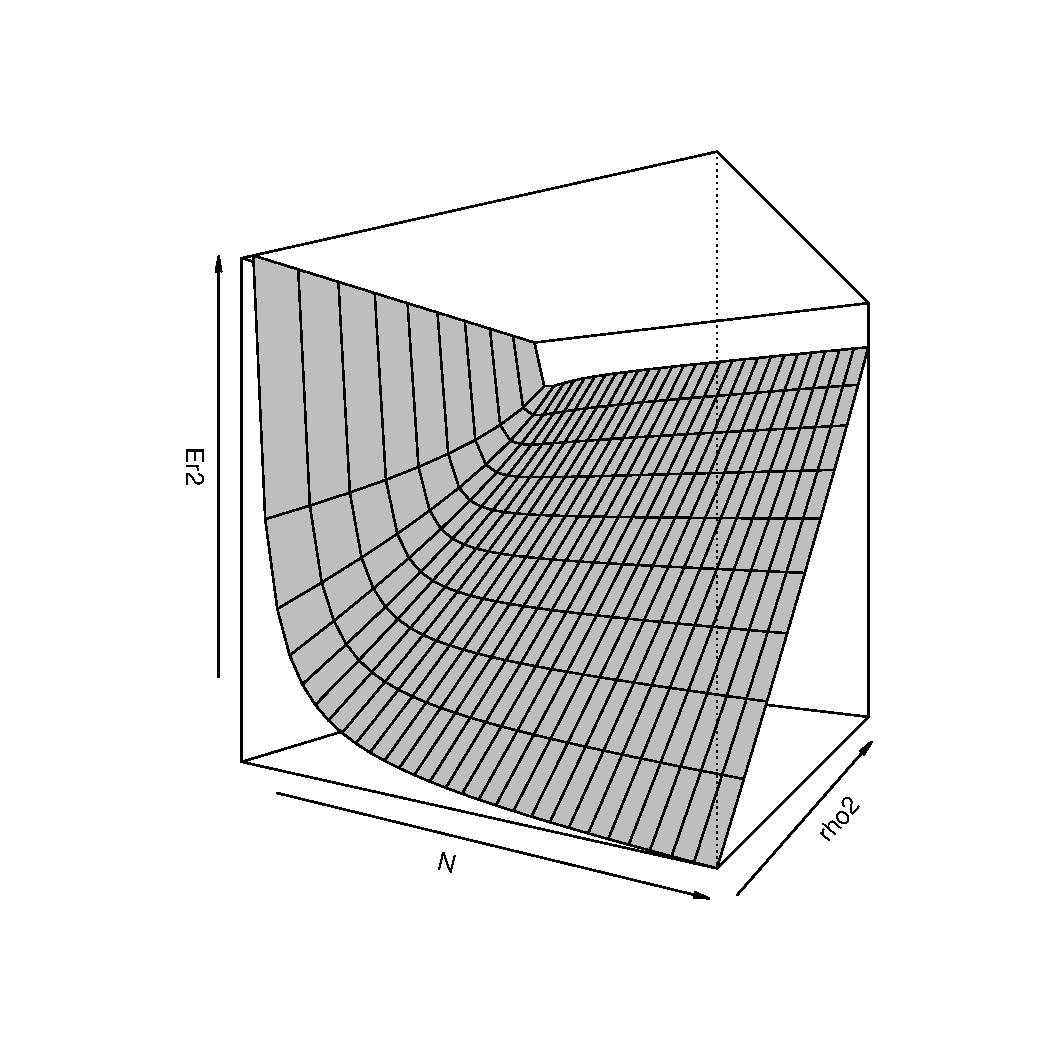
\includegraphics{2016_w11_files/figure-latex/unnamed-chunk-3-1.pdf}

Vi ser av bilderna att vi också borde ha en lägre gräns för \(/p\)
kanske för att det alls ska vara meningsfullt att titta på detta.

Kallar (Claudy 1978):s formel för Claudy formula-3.

Identifierar också 9 st formler för \(R_c\) (cross-validity coefficient)
som jag inte återger lika noggrant. En del av dessa formler utgår i sin
tur från \(\rho^2\) men skattar då denna i sin tur via atningen (Wherry
1931) eller (Olkin and Pratt 1958).

Här såekuleras även kring att en formel kan ha missförståts pga tryckfel
(blandat ihop + och -).

Simulerar för
\(\rho = .2, .5, .8, p = 2, 4, 8, N = 20, 40, 60, 100, 200\).

Nämner att (Claudy 1978) konstaterat att multikolinearitet inte haft ngn
större effekt i sammanhanget men detta tas ändå med som en faktor i
denna undersökning. Intercorrelation mellan independent variables sattes
till \(.10, .30, .50\) (samma för alls kombinationer av variabler).

Resulterade i designt experiment med
\(3 \times 3 \times 5 \times 3 = 135\) kobinationer. Upprepades 500 ggr
per kombination =\textgreater{} 67500 replicates totalt.

All data multivariat normalfördelad.

Beskriver samplingsproceduren i SAS.

Jämförde mean och sd för alla metoder baserat på de 500 repetitionerna.
Antar att skattning unbiased om mean inom \(R \in [\rho \pm 0.01]\).
Presenterar andel unbiased för olika metoder. Uppställningen är tydlig
och klar och här framkommer att Pratt bäst och att den vanliga formlen
inte särskilt bra. Bäst resultat ges då \(N/p\) stor.

Observera att (Skidmore and Thompson 2011) refererar även till denna
artikel men att deras resultat är att den vanliga formeln är OK men även
de menar att Pratt egentligen är bäst! Skidmore har även \(N=10\) och
inkluderar även skeva fördel Osäker på hur denna skillnad uppstår. En
skillnad är förstås att Skidmore inte bara tittar på normalfördelad data
utan även skeva fördelningar etc. Man gör även lite noggrannare analys
av bias (mer än att bara konstatera huruvida ett estimat kan betraktas
som unbiased eller inte).

Här gjordes också en variansanalys av bias med slutsatser. Både enskilda
och interaktinssammanslagna faktorer visar sig kunna förklara väldigt
små andelar av den totala variationen men viktigaste till minst viktiga
är \(N, \rho^2, N\rho^2, p, Np, N\rho^2p\). Andelen förklarad varians är
större för de empiriska metoderna. Allra viktigast är dock förhållandet
\(N/p\) och inte ngn enskild parameter.

Skriver att den vanliga formeln lika bra som övriga endast då
\(N/p \approx 100\). (Skidmore and Thompson 2011) är alltså lite
snällare och säger att den vanliga formeln är OK (men säger inte att den
skulle vara jättebra).

Observera att det enda vi kollar i denna artikel ju är andelen unbiased
enl def medan Skidmore undersöker mer än så (vilket de också själva
påpekar).

På det hela taget en välskriven och mkt intressant artikel.

\subsection{Läsning av (Bobko 2001)}\label{lasning-av-bobko2001}

OBS! Om \(\rho\), inte \(\rho^2\)

Detta är ett bokkapitell ur en bok som ev är ganska grundläggande och
som handlar enbart om correlation och regression. Kanske kan vara en
poäng att referera till denna för en allra första introduktion föär
ovana läsare?

Gör skillnad på två olika skrivsätt där:

\[r_{X,Y} = \frac{\sum(X - \bar{X})(Y - \bar{Y})}{\sqrt{\sum(X - \bar{X})^2\sum(Y-\bar{Y})^2}}\]
kallas conceptual formula och där dess algebraiska motsvarighet:
\[r_{X,Y} = \frac{\sum XY - (\sum X)(\sum Y)/n}{\sqrt{[\sum X^2 - (\sum X)^2/n][\sum Y^2 - (\sum Y)^2/n]}}\]
kallas computational formula. Den första lättare att tolka, den andra
att beräkna.

Påpekar att \(r\) inte är robust utan att outliers kan påverka dess
värde opropertionerligt mkt. Detta är väl antagligen också värt att
nämnas i sammanhanget då små stickprov diskuteras.

Jag läser inte färdigt denna text!

\subsection{Läsning av (Shieh 2010)}\label{lasning-av-shieh2010}

Kommer här fram till att vanliga r trots allt kan vara bättre än
unbiased versioner. Obs \(\rho\), ej \(\rho^2\). Undersöker:
\[RMSE = \sqrt{MSE(\hat{\rho}, \rho)} =\sqrt{E[(\hat{\rho} - \rho)^2]} = Bias(\hat{\rho}, \rho)^2 + Var(\hat{\rho})\].

Fig 1 och 2 ger rätt snygga illustrationer över förhållande mellan
\(\rho\) och bias resp RMSE. Lätt att se mönstret! Olika linjer för
olika n, \(n = 20, 50, 100\).

Tycker att sample \(r\) duger för \(\mid \rho \mid \leq .6\). Detta
motiveras bl a med att det är beräkningsmässigt fördelaktigt jmfrt med
olika adjusted versioner.

\subsubsection{\texorpdfstring{För
\(\rho^2\)}{För \textbackslash{}rho\^{}2}}\label{for-rho2}

OBS! Gäller \(r^2\), ej \(R^2\), dvs simple correlation, ej multiple.

\(Bias(r^2, \rho^2) > 0\) for \(0 \leq \rho \leq .70\) and
\(Bias(r^2, \rho^22) < 0\) for \(\rho \geq .75\).

Finner att för adjusted enl (Wherry 1931) \(\hat{\rho}_E^2\) (egen
beteckning) och enl Pratt \(\hat{\rho}^2_{PA}\) gäller (då \(p = 1\)):

\begin{quote}
According to these findings, \(\hat{\rho}_E^2\) is advantageous in MSE
for small \(\rho <.30\), \(r^2\) dominates for \(.30\leq \rho \leq .85\)
and \(\hat{\rho}^2_{PA}\) performs best for large \(\rho > .85\).
\end{quote}

\subsection{Läsning av (Wang and Thompson
2007)}\label{lasning-av-wang2007}

Denna artikels upplägg liknar väldigt mkt (Skidmore and Thompson 2011)
men för lite färre formler. Dock finns även här olika föfrdelningar med
olika kurtosis etc. Skidmore refererade till denna artikel och utgav sig
just för att vara en förbättring i förhållande till denna.

Slutsats att \(R^2\) bara är marginellt bias och att Smiths och (Ezekiel
and Mordecai 1929) duger bra för korrigering.

Poängterar att många tidsskrifter nu kräver rapportering av effect size.
Skriver att alla effektmått baserade på OLS kommer att överestimera sitt
sanna värde då man får en sorts over fitting ty man får in sample bias.

Så här kan man citera de olika justerade:

\begin{quote}
For example, in the R2 arena, the six primary correction candidates were
proposed by Ezekiel (1929, 1930), Smith (as cited in Ezekiel, 1929,
p.~100), Wherry (1931), Olkin and Pratt (1958), Pratt (personal
communication, October 20, 1964, cited in Claudy, 1978), and Claudy
(1978).
\end{quote}

Annan bra förklarande text till varför storleken av \(\rho\) påverkar
skattningen av sig själv:

\begin{quote}
Although the reasons why sample size and the number of measured
variables impact sampling error are intuitively straightforward, least
obvious is the reason population effect size impacts sampling error in
estimating effect sizes. Thomp- son (2002) explained, As an extreme
heuristic example, pretend that one was conducting a bivariate r2 study
in a situation in which the population r2 value was 1.0. In this
population scat- tergram, every person's asterisk is exactly on a single
regression line. In this in- stance, even if the researcher draws
ridiculously small samples, such as n = 2 or n = 3, and no matter which
participants are drawn, the researcher simply cannot incor- rectly
estimate the variance-accounted-for effect size. That is, any two or
three or four people will always define a straight line in the sample
scattergram, and thus r2 will always be 1.0. (p.~68)
\end{quote}

\section{2016-03-15}\label{section-1}

Möte med SN:

\begin{enumerate}
\def\labelenumi{\arabic{enumi}.}
\tightlist
\item
  Artikeln bör vara då fokuserad som möjligt på ett ``budskap''
\item
  Används de referenser som känns relevanta men inkludera inte ref bara
  för sakens skull.
\item
  Gör simulering med bivariat normalfördelad data och
  \(\rho^2 = .1, .25, .5, .9, N = 5, 10, 20, 30, 40, 50, 100, 150, 200\)
  upprepa 1000 ggr. 4 grafer (2 * 2) med stickprov på x-axeln och
  \(\rho^2, R^2\) på y-axeln. Olika linjer för de sex sedan tidigare
  presenterade justerade \(R^2\)-värdena, ojusterade samt väntevärdet
  enl
\end{enumerate}

Implementerar funktioner för medelvärde och varians av \(R^2\) enl
(Wishart, Kondo, and Elderton 1931):

\begin{Shaded}
\begin{Highlighting}[]
\CommentTok{# mean av R^2 enl (i)}
\NormalTok{mean_r2 <-}\StringTok{ }\NormalTok{function(rho2, n, p) \{}
  \DecValTok{1} \NormalTok{-}\StringTok{ }\NormalTok{((n -}\StringTok{ }\NormalTok{p) /}\StringTok{ }\NormalTok{(n -}\StringTok{ }\DecValTok{1}\NormalTok{)) *}\StringTok{ }\NormalTok{(}\DecValTok{1} \NormalTok{-}\StringTok{ }\NormalTok{rho2) *}\StringTok{ }\KeywordTok{Re}\NormalTok{(hypergeo::}\KeywordTok{hypergeo}\NormalTok{(}\DecValTok{1}\NormalTok{, }\DecValTok{2}\NormalTok{, .}\DecValTok{5} \NormalTok{*}\StringTok{ }\NormalTok{(n +}\StringTok{ }\DecValTok{1}\NormalTok{), rho2))}
\NormalTok{\}}

\CommentTok{# var av R^2 enl (ii)}
\NormalTok{var_r2 <-}\StringTok{ }\NormalTok{function(rho2, n, p) \{}
  \NormalTok{(}
    \NormalTok{(((n -}\StringTok{ }\NormalTok{p) *}\StringTok{ }\NormalTok{(n -}\StringTok{ }\NormalTok{p +}\StringTok{ }\DecValTok{2}\NormalTok{)) /}\StringTok{ }\NormalTok{((n -}\StringTok{ }\DecValTok{1}\NormalTok{) *}\StringTok{ }\NormalTok{(n +}\StringTok{ }\DecValTok{1}\NormalTok{))) *}\StringTok{ }
\StringTok{      }\NormalTok{(}\DecValTok{1} \NormalTok{-}\StringTok{ }\NormalTok{rho2) *}\StringTok{ }
\StringTok{      }\KeywordTok{Re}\NormalTok{(hypergeo::}\KeywordTok{hypergeo}\NormalTok{(}\DecValTok{2}\NormalTok{, }\DecValTok{2}\NormalTok{, .}\DecValTok{5} \NormalTok{*}\StringTok{ }\NormalTok{(n +}\StringTok{ }\DecValTok{3}\NormalTok{), rho2))}
  \NormalTok{) -}\StringTok{ }\NormalTok{(}\DecValTok{1} \NormalTok{-}\StringTok{ }\KeywordTok{mean_r2}\NormalTok{(rho2, n, p)) ^}\StringTok{ }\DecValTok{2}
\NormalTok{\}}
\end{Highlighting}
\end{Shaded}

Implementerar även funktioner för olika justerade \(R^2\)-värden: smith,
ezekiel, wherry, olkin\_pratt1, pratt, claudy enl (Yin and Fan 2001).
olkin\_pratt enl (Olkin and Pratt 1958). olkin\_pratt2 enl (Cattin 1980)
där olkin\_pratt1 och 2 är approximationer av olkin\_pratt

\begin{Shaded}
\begin{Highlighting}[]
\NormalTok{adjusted_r2 <-}\StringTok{ }\NormalTok{function(r2, n, p, }\DataTypeTok{adj =} \KeywordTok{c}\NormalTok{(}\StringTok{"smith"}\NormalTok{, }\StringTok{"ezekiel"}\NormalTok{, }\StringTok{"wherry"}\NormalTok{, }\StringTok{"olkin_pratt"}\NormalTok{, }\StringTok{"olkin_pratt1"}\NormalTok{, }
                                          \StringTok{"olkin_pratt2"}\NormalTok{, }\StringTok{"pratt"}\NormalTok{, }\StringTok{"claudy"}\NormalTok{)) \{}
  
  \NormalTok{smith        <-}\StringTok{ }\NormalTok{function() }\DecValTok{1} \NormalTok{-}\StringTok{ }\NormalTok{(n       /}\StringTok{ }\NormalTok{(n -}\StringTok{ }\NormalTok{p))     *}\StringTok{ }\NormalTok{(}\DecValTok{1} \NormalTok{-}\StringTok{ }\NormalTok{r2)}
  \NormalTok{ezekiel      <-}\StringTok{ }\NormalTok{function() }\DecValTok{1} \NormalTok{-}\StringTok{ }\NormalTok{((n -}\StringTok{ }\DecValTok{1}\NormalTok{) /}\StringTok{ }\NormalTok{(n -}\StringTok{ }\NormalTok{p -}\StringTok{ }\DecValTok{1}\NormalTok{)) *}\StringTok{ }\NormalTok{(}\DecValTok{1} \NormalTok{-}\StringTok{ }\NormalTok{r2)}
  \NormalTok{wherry       <-}\StringTok{ }\NormalTok{function() }\DecValTok{1} \NormalTok{-}\StringTok{ }\NormalTok{((n -}\StringTok{ }\DecValTok{1}\NormalTok{) /}\StringTok{ }\NormalTok{(n -}\StringTok{ }\NormalTok{p    )) *}\StringTok{ }\NormalTok{(}\DecValTok{1} \NormalTok{-}\StringTok{ }\NormalTok{r2)}
  \NormalTok{olkin_pratt  <-}\StringTok{ }\NormalTok{function() }\DecValTok{1} \NormalTok{-}\StringTok{ }\NormalTok{(((n -}\StringTok{ }\DecValTok{3}\NormalTok{) *}\StringTok{ }\NormalTok{(}\DecValTok{1} \NormalTok{-}\StringTok{ }\NormalTok{r2)) /}\StringTok{ }\NormalTok{(n -}\StringTok{ }\NormalTok{p -}\StringTok{ }\DecValTok{1}\NormalTok{)) *}\StringTok{ }\KeywordTok{Re}\NormalTok{(hypergeo::}\KeywordTok{hypergeo}\NormalTok{(}\DecValTok{1}\NormalTok{, }\DecValTok{1}\NormalTok{, (n -}\StringTok{ }\NormalTok{p +}\StringTok{ }\DecValTok{1}\NormalTok{) /}\StringTok{ }\DecValTok{2}\NormalTok{, }\DecValTok{1} \NormalTok{-}\StringTok{ }\NormalTok{r2))}
  \NormalTok{olkin_pratt1 <-}\StringTok{ }\NormalTok{function() }\DecValTok{1} \NormalTok{-}\StringTok{ }\NormalTok{(((n -}\StringTok{ }\DecValTok{3}\NormalTok{) *}\StringTok{ }\NormalTok{(}\DecValTok{1} \NormalTok{-}\StringTok{ }\NormalTok{r2)) /}\StringTok{ }\NormalTok{(n -}\StringTok{ }\NormalTok{p -}\StringTok{ }\DecValTok{1}\NormalTok{)) *}\StringTok{  }\NormalTok{(}\DecValTok{1} \NormalTok{+}\StringTok{ }\NormalTok{(}\DecValTok{2} \NormalTok{*}\StringTok{ }\NormalTok{(}\DecValTok{1} \NormalTok{-}\StringTok{ }\NormalTok{r2)) /}\StringTok{ }\NormalTok{(n -}\StringTok{ }\NormalTok{p -}\StringTok{ }\DecValTok{1}\NormalTok{))}
  \NormalTok{olkin_pratt2 <-}\StringTok{ }\NormalTok{function() }\DecValTok{1} \NormalTok{-}\StringTok{ }\NormalTok{(((n -}\StringTok{ }\DecValTok{3}\NormalTok{) *}\StringTok{ }\NormalTok{(}\DecValTok{1} \NormalTok{-}\StringTok{ }\NormalTok{r2)) /}\StringTok{ }\NormalTok{(n -}\StringTok{ }\NormalTok{p -}\StringTok{ }\DecValTok{1}\NormalTok{)) *}\StringTok{ }\NormalTok{((}\DecValTok{1} \NormalTok{+}\StringTok{ }\NormalTok{(}\DecValTok{2} \NormalTok{*}\StringTok{ }\NormalTok{(}\DecValTok{1} \NormalTok{-}\StringTok{ }\NormalTok{r2)) /}\StringTok{ }\NormalTok{(n -}\StringTok{ }\NormalTok{p -}\StringTok{ }\DecValTok{1}\NormalTok{)) +}\StringTok{ }
\StringTok{                                 }\NormalTok{((}\DecValTok{8} \NormalTok{*}\StringTok{ }\NormalTok{(}\DecValTok{1} \NormalTok{-}\StringTok{ }\NormalTok{r2) ^}\StringTok{ }\DecValTok{2}\NormalTok{)   /}\StringTok{ }\NormalTok{((n -}\StringTok{ }\NormalTok{p -}\StringTok{ }\DecValTok{1}\NormalTok{) *}\StringTok{  }\NormalTok{(n -}\StringTok{ }\NormalTok{p +}\StringTok{ }\DecValTok{3}\NormalTok{))))}
  \NormalTok{pratt        <-}\StringTok{ }\NormalTok{function() }\DecValTok{1} \NormalTok{-}\StringTok{ }\NormalTok{(((n -}\StringTok{ }\DecValTok{3}\NormalTok{) *}\StringTok{ }\NormalTok{(}\DecValTok{1} \NormalTok{-}\StringTok{ }\NormalTok{r2)) /}\StringTok{ }\NormalTok{(n -}\StringTok{ }\NormalTok{p -}\StringTok{ }\DecValTok{1}\NormalTok{)) *}\StringTok{  }\NormalTok{(}\DecValTok{1} \NormalTok{+}\StringTok{ }\NormalTok{(}\DecValTok{2} \NormalTok{*}\StringTok{ }\NormalTok{(}\DecValTok{1} \NormalTok{-}\StringTok{ }\NormalTok{r2)) /}\StringTok{ }\NormalTok{(n -}\StringTok{ }\NormalTok{p -}\StringTok{ }\FloatTok{2.3}\NormalTok{))}
  \NormalTok{claudy       <-}\StringTok{ }\NormalTok{function() }\DecValTok{1} \NormalTok{-}\StringTok{ }\NormalTok{(((n -}\StringTok{ }\DecValTok{4}\NormalTok{) *}\StringTok{ }\NormalTok{(}\DecValTok{1} \NormalTok{-}\StringTok{ }\NormalTok{r2)) /}\StringTok{ }\NormalTok{(n -}\StringTok{ }\NormalTok{p -}\StringTok{ }\DecValTok{1}\NormalTok{)) *}\StringTok{  }\NormalTok{(}\DecValTok{1} \NormalTok{+}\StringTok{ }\NormalTok{(}\DecValTok{2} \NormalTok{*}\StringTok{ }\NormalTok{(}\DecValTok{1} \NormalTok{-}\StringTok{ }\NormalTok{r2)) /}\StringTok{ }\NormalTok{(n -}\StringTok{ }\NormalTok{p -}\StringTok{ }\DecValTok{1}\NormalTok{))}
  
  \NormalTok{x <-}\StringTok{ }\KeywordTok{vapply}\NormalTok{(adj, do.call, }\KeywordTok{numeric}\NormalTok{(}\DecValTok{1}\NormalTok{), }\KeywordTok{list}\NormalTok{(), }\DataTypeTok{envir =} \KeywordTok{environment}\NormalTok{())}
  \KeywordTok{names}\NormalTok{(x) <-}\StringTok{ }\NormalTok{adj}
  \NormalTok{x}
\NormalTok{\}}

\NormalTok{r2 <-}\StringTok{ }\NormalTok{function(x, rho2, ...) \{}
  \NormalTok{r2 <-}\StringTok{ }\KeywordTok{summary}\NormalTok{(x)$r.squared}
  \NormalTok{n  <-}\StringTok{ }\KeywordTok{length}\NormalTok{(}\KeywordTok{residuals}\NormalTok{(x))}
  \NormalTok{p  <-}\StringTok{ }\KeywordTok{length}\NormalTok{(x$coefficients) -}\StringTok{ }\DecValTok{1}
  
  \KeywordTok{c}\NormalTok{(}\DataTypeTok{r2 =} \NormalTok{r2, }\DataTypeTok{mean_r2 =} \KeywordTok{mean_r2}\NormalTok{(rho2, n, p), }\DataTypeTok{var_r2 =} \KeywordTok{var_r2}\NormalTok{(rho2, n, p),}
         \KeywordTok{adjusted_r2}\NormalTok{(r2, n, p, ...))}
\NormalTok{\}}
\end{Highlighting}
\end{Shaded}

Har nu implementerat funktionerna ovan i \texttt{r2samplesize}-paketet
och kan därmed framöver anropa dem därifrån.

\section{2016-03-17}\label{section-2}

Jobbade med Teds projekt.

\section{2016-03-18}\label{section-3}

Catched up on Pocket etc.

\subsection{Läsning av (Croux and Dehon
2003)}\label{lasning-av-croux2003}

Tolkar nämnaren i formeln för \(R^2\) som residualvarians för modell med
enbart intercept.

UNdersöker robustness av \(R^2\), dvs hur enskilda outliers påverkar.
Finns föreslagna robusta skattningar av \(R^2\) sedan tidigare som inte
bygger på (men som kan fås till) till den vanliga LS-skattningen under
vissa förhållanden.

I huvudsak väldigt teoretiskt och torr men ändå med det viktiga
budskapet att den vanliga LS-skattnigen inte är robust.

\subsection{Läsning av (Renaud and Victoria-Feser
2010)}\label{lasning-av-renaud2010}

Handlar också om robusthet. Observera att vi tidigare sett att \(R^2\)
är ganska robust avseende ev skevhet i underliggande fördelning men vi
är väl helt enkelt känsligarte för outliers än för det.

Det finns många olika förslag på robusta estimators, även för små
stickprtovsstorlekar. DOck hade man hittils inte undersökt dem empiriskt
med simuleringar etc, vilket sker i denna artikel.

Noterar att \(R^2\) avser korrelation mellan y och bästa möjliga
linjärkobination av x (eftersom ju alla sådana linjärkombinatioer har
samma korrelation).

\begin{quote}
It is important to note that normality is not assumed, merely the
existence of the second moments. Compared to covariance penalty methods,
although the R2 is solely based on the covariance penalty, it plays an
important role in model fit assessment. It should certainly not be used
as a unique model fit assessor, but can provide a reasonable and rapid
model fit indication.
\end{quote}

\begin{quote}
The R2 is usually presented as the quantity that estimates the
percentage of variance of the response variable explained by its
(linear) relationship with the explanatory variables.
\end{quote}

Gör simuleringar med lite blandade data, kontinuerliga ovh
dummy-variabler. Testar 8 olika estimat.

Man kan ju iofs också tänka att en utliggare är verklig och att
korrelation bara ska mäta linjärt samband, vilket man kanske alltså inte
har fullt ut ifall även utliggare ska kunna förklaras mha av modellen???

\subsection{Läsning av (Asuero, Sayago, and González
2006)}\label{lasning-av-asuero2006}

Poängterar att korrelation och regression mäter olika saker.

\begin{quote}
For either correlation or for regression models, the same expressions
are valid, although they differ significantly in meaning.
\end{quote}

Nämner också att skattningen inte robust men att Spearmans korrelation
då är ett alternativ som bara tar hänsyn till ranking och inte exakta
värden.

F.ö. en mkt bra, grundläggande och översiktlig artikel som kan
rekommenderas som en första introduktion till ämnet i största allmänhet!

\begin{quote}
The correlation coefficient, r, is a standardized index for which the
value does not depend on the measurement scales of the variables. Its
values lies (58) in the range (-1, 1), and its squared value describes
(59) the proportional reduction in variability of one variable when the
other is held constant. It is worth noting that since for any r2 other
than 0 or 1, \textbar{}r2\textbar{}\textless{}r; r may give the
impression of a closer relationship (60) between x and y than does the
corresponding r2. Therefore, although the correlation coefficient is by
itself an important measure of relationship between the variables, it is
R squared that permits comparison of the strengths of relationships. The
reasons for making a distinction (41, 5) between r and R are that i) r
is a measure of association between two random variables, whereas R is a
measure between a random variable y and its prediction y from a
regression model; ii) R is always well defined, regardless of whether
the independent variable assumed to be random or fixed. In contrast,
calculating the correlation between a random variable, y, and a fixed
predictor variable x, that is, a variable that is not considered random,
makes no sense.
\end{quote}

\begin{quote}
Because r2 gives the proportion of variance that is common between the
two variables x and y, the uncommon or unique variance is the remainder,
and this is known as the coefficient of nondetermination and is usually
symbolized as k2=1 - r2. Some statisticians refer to (61) the
coefficient of alienation k, which indicates the degree of lack of
relationship.
\end{quote}

\subsection{Läsning av (Hössjer 2008)}\label{lasning-av-hossjer2008}

OBS! Skriven av en Stockholmare! :-)

Handlar om mixed models. Kanske värt att nämna i ev samband med fixed
och random models? Men känns i övrigt lite off topic vilket gör att jag
inte läser mer än abstract.

\subsection{Läsning av (Burton et al.
2006)}\label{lasning-av-burton2006}

OBS! Handlar inte om ämnet utan om design av simulationsstudier inom
medecin.

Föreslår att man vid simuleringsstudier, likväl som vid RCT etc
upprättar ett studieprotokoll och att alla val av storlekar och metoder
etc motiveras väl. Se fig 1 för uppställning av vad man bör tänka på.
Man bör ange vilken slumptalsgenerator och med vilken seed som används.
Måste tänka på hur olika variabler korrelerar, ofta orimligt att
verkligen ha helt okorrelerade data. Bör om möjligt undersöka hela
paramterspejset eller åtm den del som är av intresse vid tillämpning.

Olika mått för performance mearure kan och bör rapporteras, utöver ren
bias även andel bias av hela måttet, standardiserad bias, MSE etc.

Genomgång har visat att väldigt många simuleringsstudier är undermåligt
beskrivna. Skärpning!

\section*{Referenser}\label{referenser}
\addcontentsline{toc}{section}{Referenser}

\hypertarget{refs}{}
\hypertarget{ref-Asuero2006}{}
Asuero, a. G., A. Sayago, and a. G. González. 2006. ``The Correlation
Coefficient: An Overview.'' \emph{Critical Reviews in Analytical
Chemistry} 36 (July): 41--59.
doi:\href{https://doi.org/10.1080/10408340500526766}{10.1080/10408340500526766}.

\hypertarget{ref-Bobko2001}{}
Bobko, Philip. 2001. ``A Review of the Correlation Coefficient and its
Properties.'' In \emph{Correlation and Regression: Applications for
Industrial Organizational Psychology and Management.}, 12--42.
doi:\href{https://doi.org/10.4135/9781412983815}{10.4135/9781412983815}.

\hypertarget{ref-Burton2006}{}
Burton, Andrea, Douglas G. Altman, Patrick Royston, and Roger L. Holder.
2006. ``The design of simulation studies in medical statistics.''
\emph{Statistics in Medicine} 25: 4279--92.
doi:\href{https://doi.org/10.1002/sim.2673}{10.1002/sim.2673}.

\hypertarget{ref-Cattin1980}{}
Cattin, Philippe. 1980. ``Estimation of the Predictive Power of a
Regression Model.'' \emph{Journal of Applied Psychology} 65 (4):
407--14.
doi:\href{https://doi.org/10.1037//0021-9010.65.4.407}{10.1037//0021-9010.65.4.407}.

\hypertarget{ref-Claudy1978}{}
Claudy, J. G. 1978. ``Multiple Regression and Validity Estimation in One
Sample.'' \emph{Applied Psychological Measurement} 2 (4): 595--607.
doi:\href{https://doi.org/10.1177/014662167800200414}{10.1177/014662167800200414}.

\hypertarget{ref-Croux2003}{}
Croux, Cristophe, and Catherine Dehon. 2003. ``Estimators of the
multiple correlation coefficient: Local robustness and confidence
intervals.'' \emph{Statistical Papers} 44 (3): 315--34.
doi:\href{https://doi.org/10.1007/s00362-003-0158-7}{10.1007/s00362-003-0158-7}.

\hypertarget{ref-Ezekiel1929}{}
Ezekiel, and Mordecai. 1929. ``The Application of the Theory of Error to
Multiple and Curvilinear Correlation.'' \emph{Journal of the American
Statistical Association} 24 (165): 99--104.

\hypertarget{ref-Hossjer2008}{}
Hössjer, Ola. 2008. ``On the coefficient of determination for mixed
regression models.'' \emph{Journal of Statistical Planning and
Inference} 138 (10): 3022--38.
doi:\href{https://doi.org/10.1016/j.jspi.2007.11.010}{10.1016/j.jspi.2007.11.010}.

\hypertarget{ref-Olkin1995}{}
Olkin, Ingram, and Jeremy D. Finn. 1995. ``Correlations redux.''
\emph{Psychological Bulletin} 118 (1): 155--64.

\hypertarget{ref-Olkin1958}{}
Olkin, Ingram, and J.W. Pratt. 1958. ``Unbiased estimation of certain
correlation coefficients.'' \emph{The Annals of Mathematical Statistics}
29 (1): 201--11.
doi:\href{https://doi.org/10.2307/2237306}{10.2307/2237306}.

\hypertarget{ref-Renaud2010}{}
Renaud, Olivier, and Maria Pia Victoria-Feser. 2010. ``A robust
coefficient of determination for regression.'' \emph{Journal of
Statistical Planning and Inference} 140 (7). Elsevier: 1852--62.
doi:\href{https://doi.org/10.1016/j.jspi.2010.01.008}{10.1016/j.jspi.2010.01.008}.

\hypertarget{ref-Shieh2010}{}
Shieh, Gwowen. 2010. ``Estimation of the simple correlation
coefficient.'' \emph{Behavior Research Methods} 42 (4): 906--17.
doi:\href{https://doi.org/10.3758/BRM.42.4.906}{10.3758/BRM.42.4.906}.

\hypertarget{ref-Skidmore2011}{}
Skidmore, Susan Troncoso, and Bruce Thompson. 2011. ``Choosing the Best
Correction Formula for the Pearson r 2 Effect Size.'' \emph{The Journal
of Experimental Education} 79 (3): 257--78.
doi:\href{https://doi.org/10.1080/00220973.2010.484437}{10.1080/00220973.2010.484437}.

\hypertarget{ref-Wang2007}{}
Wang, Zhongmiao, and Bruce Thompson. 2007. ``Is the Pearson r 2 Biased,
and if So, What Is the Best Correction Formula?'' \emph{The Journal of
Experimental Education} 75 (2): 109--25.
doi:\href{https://doi.org/10.3200/JEXE.75.2.109-125}{10.3200/JEXE.75.2.109-125}.

\hypertarget{ref-Wherry1931}{}
Wherry, R. 1931. ``A new formula for predicting the shrinkage of the
coefficient of multiple correlation.'' \emph{The Annals of Mathematical
Statistics} 2 (4): 440--57.
\url{http://www.jstor.org/stable/2957681$/backslash$npapers2://publication/uuid/F3D4916B-BB98-4094-A459-DF4387AC9610}.

\hypertarget{ref-Wishart1931}{}
Wishart, Author J, T Kondo, and E M Elderton. 1931. ``The Mean and
Second Moment Coefficient of the Multiple Correlation Coefficient, in
Samples from a Normal Population.'' \emph{Biometrika} 22 (3/4): 353--76.

\hypertarget{ref-Yin2001}{}
Yin, Ping, and Xitao Fan. 2001. ``Estimating R 2 Shrinkage in Multiple
Regression: A Comparison of Different Analytical Methods.'' \emph{The
Journal of Experimental Education} 69 (2): 203--24.
doi:\href{https://doi.org/10.1080/00220970109600656}{10.1080/00220970109600656}.

\end{document}
